\section{Week 1 - Foundations of Convolutional Neural Networks}
Learn to implement the foundational layers of CNNs (pooling, convolutions) and to stack them properly in a deep network to solve multi-class image classification problems.
\subsection{Convolutional Neural Networks}

\subsubsection{Computer Vision}
Example applications: Image Classification, Object detection, Neural Style Transfer.
High resolution pictures (e.g. 1000x1000px) will cause the NN to be too large as you will have a large input.  To handle so much features, you need to better implement the \textbf{convolution operation}, which is one of the fundamental building blocks of convolutional neural networks. 

\subsubsection{Edge Detection Example}
Matrix Convolutional operation: take one big matrix (e.g. A: 6x6) and multiply it by the \textbf{filter} or \textbf{mask} matrix (e.g. B: 3x3) to get a resulting matrix of (C: 4x4).
First cell of the resulting matrix is:
\begin{multline}
    C[1, 1] = A[1, 1] * B[1, 1] + A[2, 1] * B[2, 1] + A[3, 1] * B[3, 1] \\
    + A[1, 2] * B[1, 2] + A[2, 2] * B[2, 2] + A[3, 2] * B[3, 2] \\
    + A[1, 3] * B[1, 3] + A[2, 3] * B[2, 3] + A[3, 3] * B[3, 3]
\end{multline}
Then move the small matrix inside A to the right and down until all cells of C are populated.

\subsubsection{More Edge Detection}
Learning to detect edges, treat the 9 numbers of the filter matrix (i.e. 3x3) as parameters that the Backpropagation will learn them.

\subsubsection{Padding}
If A is (n, n) B is (f, f), then the convolution product is (n-f+1, n-f+1). Also the cell in the middle of A is been used many times as it overlaps many matrices, on the other hand the top left cell is used only by one matrix, information is been lost. Problems with convolutions include:
\begin{itemize}
    \item shrinking output
    \item throw away info from edge
\end{itemize}
A solution is padding or adding more cells in the corners of A. To decide how much to convolute, the are two techniques:
\begin{itemize}
    \item Valid Convolution: no padding. (n, n) * (f, f) = (n-f+1, n-f+1)
    \item Same Convolution: Pad so that output size is the same as the input size.
    \begin{equation}
        n+2p-f+1 = n => p = \frac{f - 1}{2}
    \end{equation}
\end{itemize}
In computer vision, $f$ is usually an \texttt{odd} number.

\subsubsection{Strided Convolutions}
Instead of moving the filter in A to the right or down with 1 cell, use a \texttt{stride} value (e.g. $stride = 2$).

In mathematical literature, convolution is called corss-correlation.

\subsubsection{Convolutions Over Volume}
Images have many channels, like Red, Green and Blue, the filter/mask matrix will also have same number of channels, however the resulting matrix will have only one channel.
E.g. a matrix of 6 x 6 x 3 convoluted by 3 x 3 x 3 will result in 4 x 4 x 1.

What if you wanted to use multiple filters at a time? you will just convolute every filter against the A matrix and you have as much result as filters.

Summay: (n, n, nc) * (f, f, nc) = (n-f+1, n-f+1, nc'). Where $nc$ is number of channels, and $nc'$ is the number of filters.

\subsubsection{One Layer of a Convolutional Network}
Example of building a Convolutional Neural Network: the input matrix is nothing by $A^{[i]}$ and the filter matrix becomes $W^{[i]}$. In the following equation there is a convolution product between w and a
\begin{equation}
    z^{[1]} = w^{[1]} * a^{[1]} + b^{[1]}
\end{equation}
\begin{equation}
    a^{[1]} = g(z^{[1]})
\end{equation}

\texttt{Numbers of parameters in one layer?}
If you have 10 filters that are 3x3x3 in one layer of a neural network, how many paramters does that layer have?
3x3x3 filter is 27 parameters, plus the bias, that gives 28 parameters, summing up we will have 280 parameters for the ten filters.

The number of parameters in a CNN is fixed which makes this network not overfitting.


Notation
if layer l is a convolution layer:
\begin{itemize}
    \item $f^{[l]}$ filter size
    \item $p^{[l]}$ padding
    \item $s^{[l]}$ stride
    \item $n^{[l]}_c$ number of filters
    \item Each filter is $f^{[l]}$ x $f^{[l]}$ x $n^{[l-1]}_c$
    \item Activations: $a^{[l]}$ x $n^{[l]}_w$ x $n^{[l]}_c$
$A^{[l]}$ => $M$ x $n^{[l]}_h$ x $n^{[l]}_w$ x $n^{[l]}_c$
    \item Weights: $f^{[l]}$ x $f^{[l]}$ x $n^{[l-1]}_c$ x $n^{[l]}_c$
    \item bias: $n^{[l]}_c$ - (1, 1, 1, $n^{[l]}_c$)

    \item input: $n^{[l-1]}_h$ => $n^{[l]}_h$ x $n^{[l]}_w$ x $n^{[l]}_c$
    \item Output: $n^{[l]}_h$ x $n^{[l]}_w$ x $n^{[l]}_c$, 
$n^{[l]}_h$ = $\floor*{\frac{n^{[l-1]}_h + 2 p^{[l]} - f^{[l]}} {s^{[l]}} + 1}$
\end{itemize}

\subsubsection{Simple Convolutional Network Example}
Types of layer in a convolutional network
\begin{itemize}
    \item Convolution (CONV)
    \item Pooling (POOL)
    \item Fully connected (FC)
\end{itemize}


\subsubsection{Pooling Layers}
Types of pooling:
\begin{description}
    \item[Max pooling] uses the MAX function when aggregating cells
    \item[Avg pooling] uses the AVG function when aggregating cells
\end{description}
Ex- Max pooling: for a 4x4 matrix into a 2x2 matrix, in the original matrix divide it into 2x2 regions then take the max in each of those regions which you will pass to the 2x2 output matrix.
Max pooling has hyperparameters $f$ and $s$ but no parameters for gradient to learn.

\subsubsection{CNN Example}
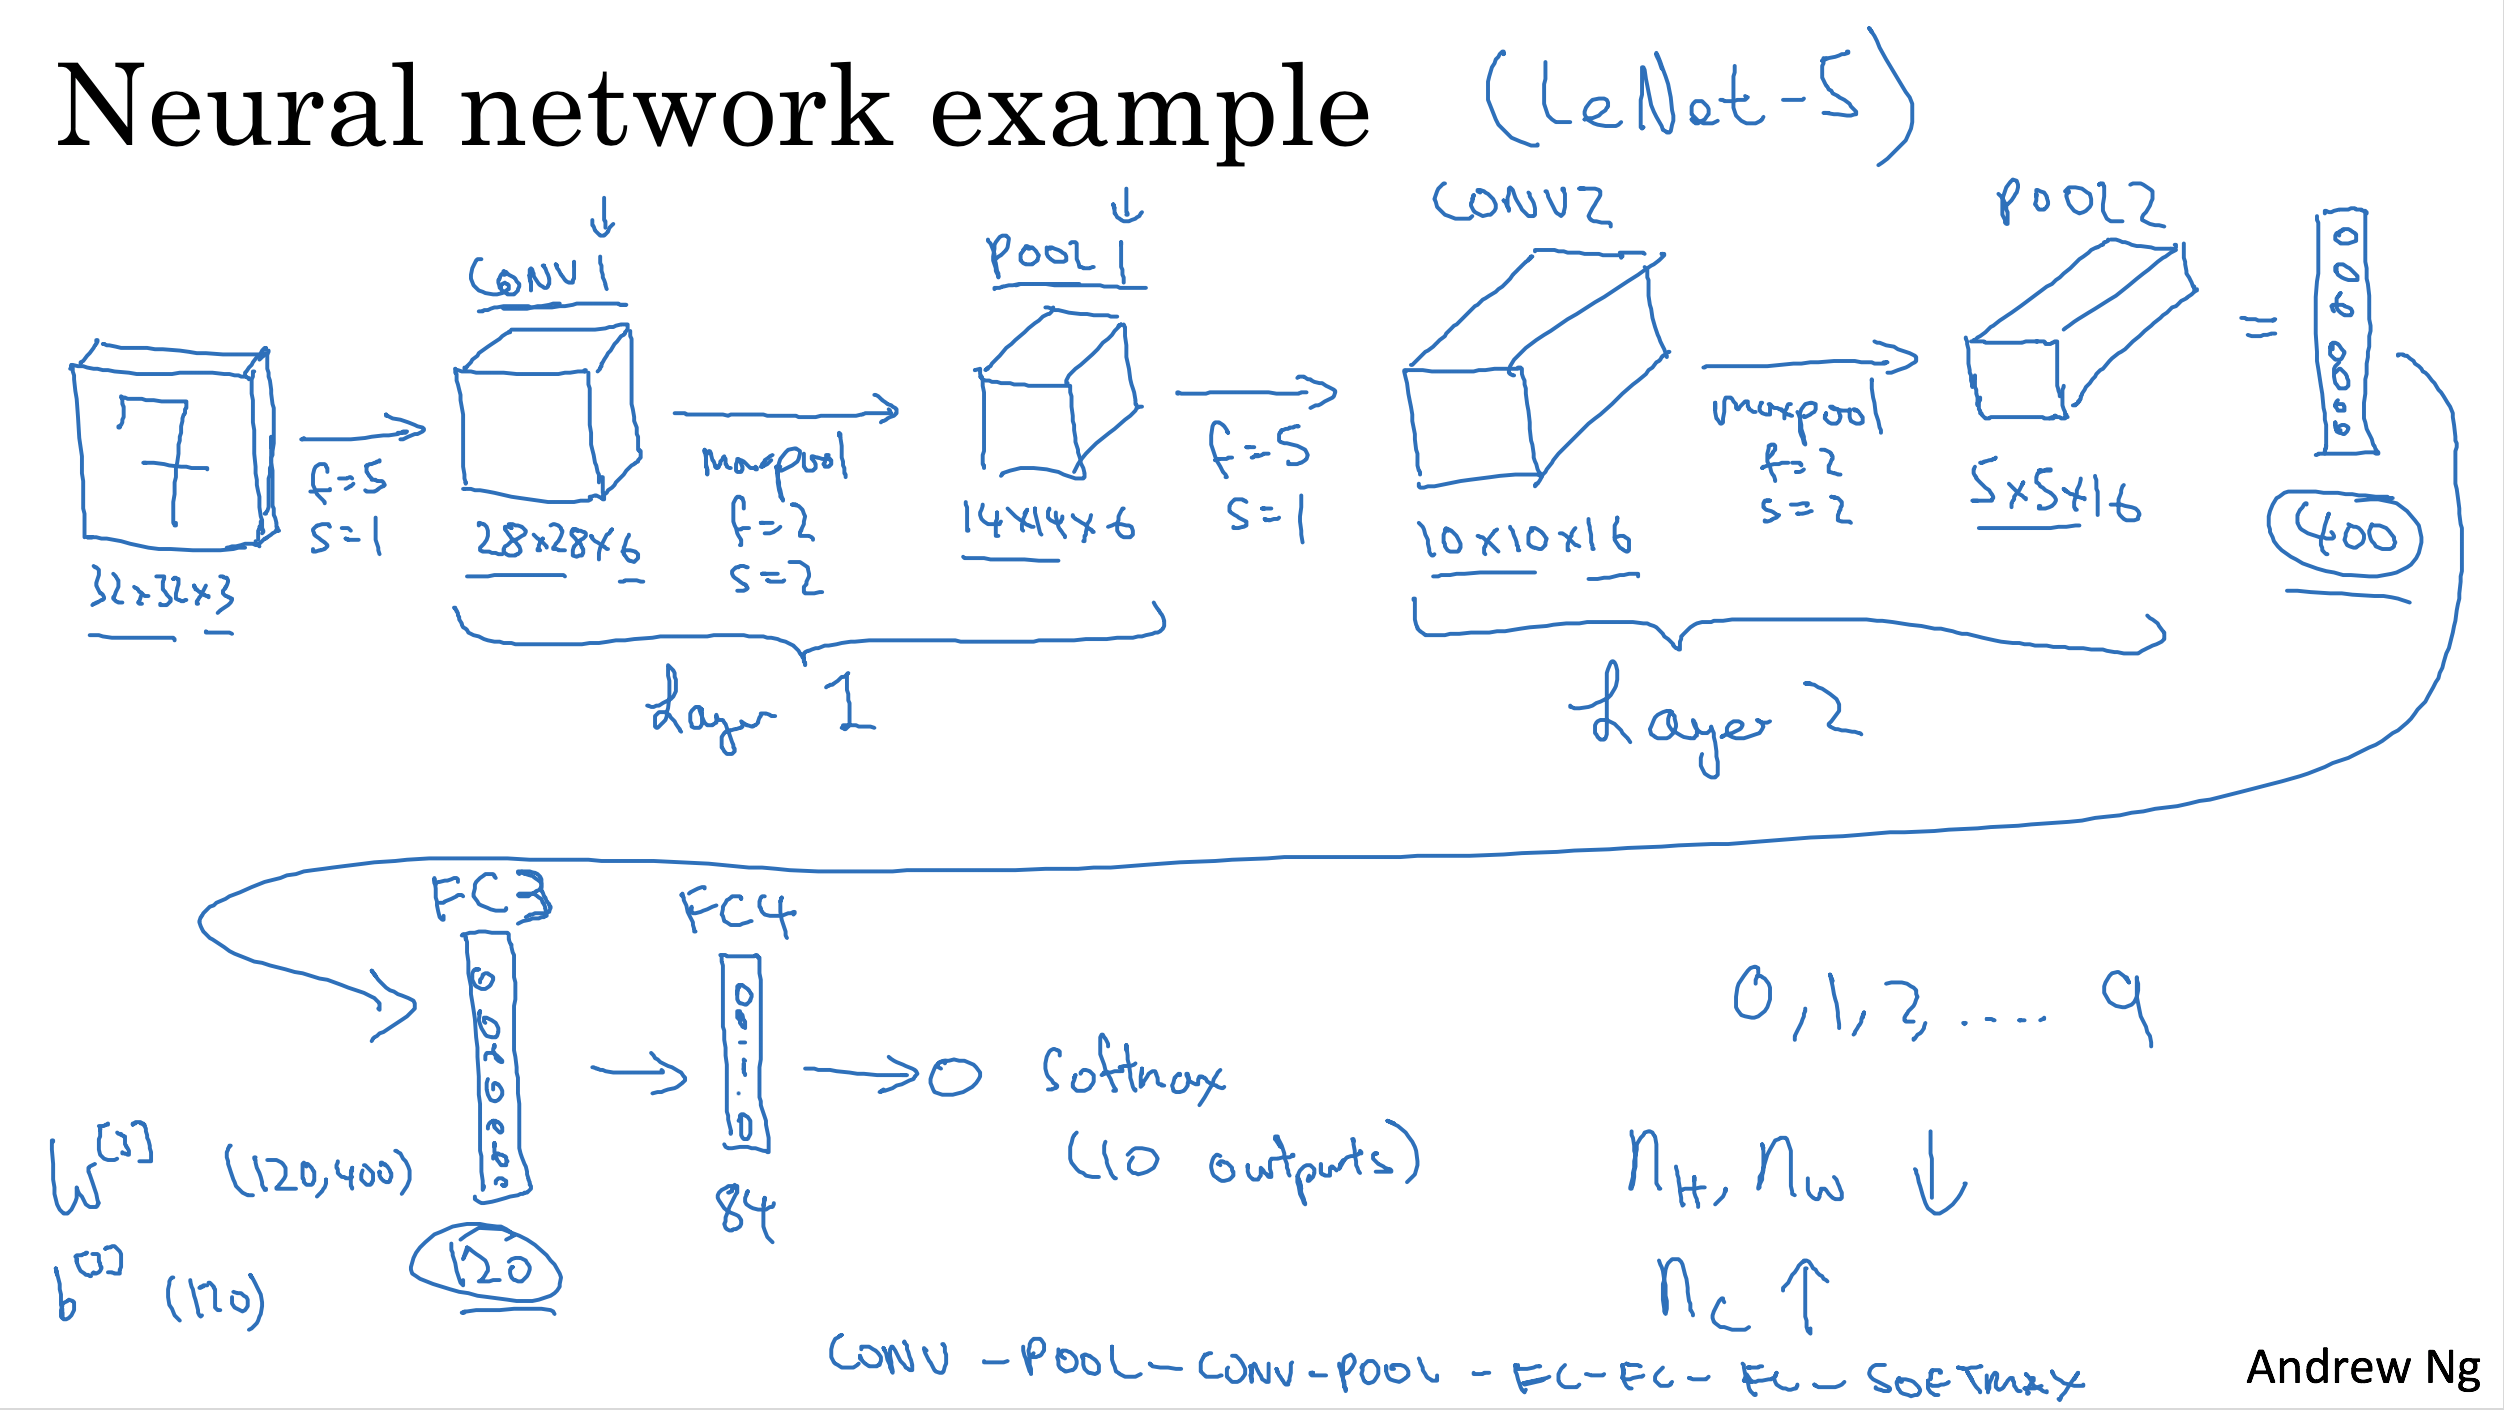
\includegraphics[scale=0.35]{CNN_Example}
\begin{center}
\begin{tabular}{ |c|c|c|c| }
 \hline
 & Activation shape & Activation Size & \# parameters \\
 \hline
 Input & (32, 32, 3) & 3 072 & 0 \\
 \hline
 CONV1 (f=5, s=1)& (28, 28, 8) & 6 272 & 208 \\
 \hline
 POOL1 & (14, 14, 8) & 1 568 & 0 \\
 \hline
 CONV2 (f=5, s=1) & (10, 10, 16) & 1 600 & 416 \\
 \hline
 POOL2 & (5, 5, 16) & 400 & 0 \\
 \hline
 FC3 & (120, 1) & 120 & 48 001 \\
 \hline
 FC4 & (84, 1) & 84 & 10 081 \\
 \hline
 Softmax & (10, 1) & 10 & 841 \\
 \hline
\end{tabular}
\end{center}
The number of parameters in the convolutional layer is relatively small, it goes up in the Fully Connected layers. The size of the activation matrix goes down as we go deeper in the NN.

\subsubsection{Why Convolutions?}
\begin{description}
    \item[Parameter sharing:] A feature detector (such as a vertical edge detector) that’s useful in one part of the image is probably useful in another part of the image.
    \item[Sparsity of connections:] In each layer, each output value depends only on a small number of inputs.
\end{description}

\subsection{Practice Questions}

\subsubsection*{QUIZ - The basics of ConvNets}
\textbf{1.} What do you think applying this filter to a grayscale image will do?
\begin{itemize}
    \item Detect horizontal edges
    \item Detect 45 degree edges (X 1)
    \item Detect image contrast (X 2)
    \item Detect vertical edges (X 3)
\end{itemize}
\textbf{2.} Suppose your input is a 300 by 300 color (RGB) image, and you are not using a convolutional network. If the first hidden layer has 100 neurons, each one fully connected to the input, how many parameters does this hidden layer have (including the bias parameters)?
\begin{itemize}
    \item 9,000,001
    \item 9,000,100
    \item 27,000,001
    \item 27,000,100 (X)
\end{itemize}
\textbf{3.} Suppose your input is a 300 by 300 color (RGB) image, and you use a convolutional layer with 100 filters that are each 5x5. How many parameters does this hidden layer have (including the bias parameters)?
\begin{itemize}
    \item 2501 (X 2) (5x5)*100+1=2501
    \item 2600 (X 1) (5x5+1)*100=2600
    \item 7500
    \item 7600
\end{itemize}
\textbf{4.} You have an input volume that is 63x63x16, and convolve it with 32 filters that are each 7x7, using a stride of 2 and no padding. What is the output volume?
\begin{itemize}
    \item 16x16x32
    \item 29x29x16
    \item 29x29x32 (X) $\floor{\frac{63+2p-f}{s}+1}=\floor{\frac{63+0-7}{2}+1}=29$
    \item 16x16x16
\end{itemize}
\textbf{5.} You have an input volume that is 15x15x8, and pad it using “pad=2.” What is the dimension of the resulting volume (after padding)?
\begin{itemize}
    \item 19x19x12
    \item 17x17x8
    \item 17x17x10
    \item 19x19x8 (X) $= 15+2p= 19$
\end{itemize}
\textbf{6.} You have an input volume that is 63x63x16, and convolve it with 32 filters that are each 7x7, and stride of 1. You want to use a “same” convolution. What is the padding?
\begin{itemize}
    \item 1
    \item 2
    \item 3 (X) $63=\floor{\frac{63+2p-f}{s}+1}=\floor{\frac{63+0-7}{1}+1}=> 0=2p-6 => p = 3$
    \item 7
\end{itemize}
\textbf{7.} You have an input volume that is 32x32x16, and apply max pooling with a stride of 2 and a filter size of 2. What is the output volume?
\begin{itemize}
    \item 32x32x8
    \item 16x16x8
    \item 16x16x16 (X) Max pool divide by 2 the original size
    \item 15x15x16
\end{itemize}
\textbf{8.} Because pooling layers do not have parameters, they do not affect the backpropagation (derivatives) calculation.
\begin{itemize}
    \item True (X 1)
    \item False (X 2)
\end{itemize}
\textbf{9.} In lecture we talked about “parameter sharing” as a benefit of using convolutional networks. Which of the following statements about parameter sharing in ConvNets are true? (Check all that apply.)
\begin{itemize}
    \item It allows a feature detector to be used in multiple locations throughout the whole input image/input volume. (X 1 2)
    \item It allows parameters learned for one task to be shared even for a different task (transfer learning). (X 1)
    \item It allows gradient descent to set many of the parameters to zero, thus making the connections sparse.
    \item It reduces the total number of parameters, thus reducing overfitting. (X 2)
\end{itemize}
\textbf{10.} In lecture we talked about “sparsity of connections” as a benefit of using convolutional layers. What does this mean?
\begin{itemize}
    \item Regularization causes gradient descent to set many of the parameters to zero.
    \item Each layer in a convolutional network is connected only to two other layers
    \item Each activation in the next layer depends on only a small number of activations from the previous layer. (X)
    \item Each filter is connected to every channel in the previous layer.
\end{itemize}